\newpage
\section{Réalisation du projet}
\label{sec:realisation}

\noindent Cette section fait écho à la section précédente \ref{sec:concept}. Ici, nous détaillerons la mise en oeuvre effective de notre conception.

\subsection{Solution moteur}

\paragraph{}
    Dans cette sous-section, nous décrirons en détail les solutions mises en place pour le gestion algorithmique du logiciel.

\subsubsection{Point de vue global}

\paragraph{}
    Il est important de préciser le fonctionnement globale de notre noyau pour bien comprendre les solutions moteurs utilisaient et leurs différents appels.

\paragraph{}  
    Notre simulation fonctionne sur une boucle principale avec notre Thread qui fait appel a chaque itération a la méthode advance de Manager. C'est a partir de la que les actions ou les déplacements seront gérés a partir d'ici par les différents managers.

\paragraph{}
    Ensuite, c'est boucle principale va être limiter dans le temps par un chronomètre qui va être incrémenter et allant jusqu'à 90 : 00, temps a partir duquel le jeu s'arrête.


\subsubsection{Système d'action}

\paragraph{}
    Ici, nous détaillerons les solutions apportées dans la classe ManagBall pour gérer les actions lors de la simulations. Nous considérons comme action, toutes interactions de joueur avec le ballon.

\paragraph{Choix d'action}
    D'abord, il serait intéressants de préciser comment est réalisé le choix d'une action. A l'intérieur de la classe, il y a un attribut qui permet le stockage des actions a réaliser, une ArrayList contenant des objet de type Action qui correspond a notre Interface pour toute nos actions. Lorsque cette attribut est vide, il faut choisir une action adapte, pour cela nous récupérons le Joueur en possession du ballon puis a partir d'un nombre important d'information, nous calculons deux scores. Premièrement, un score pour le choix d'un tir : ce score prend en compte l'avancement du joueur par rapport au but adverse, la distance par rapport au joueur adverse le plus proche, si la zone de déclenchement du tir est acceptable et enfin si le joueur est seul face au gardien. Ensuite, si le score est suffisamment haut, l'action Tir est crée et ajouter à la liste d'actions. Cependant si le score n'est pas suffisant, viens alors le calcul d'un deuxième score pour la réception d'une passe qui permet de choisir le meilleur receveur possible pour la passe qui est ensuite crée et ajoutée dans la liste.

\paragraph{}
    Évidemment, les Passe et les Tir ne sont pas les seules actions de notre simulation. Cependant les autres actions découlent directement de ces deux là. En effet, pour l'action Arrêt, l'action ne peut être tenter qu'une seule fois par Tir et en fonction de la statistique d'Arret du gardien peut amener a une corner. Pour l'action Interception, elles sont créer lorsqu'une action se situe déjà dans la liste et a chaque passage chaque joueur adverse aura la possibilité d'intercepter la balle. Les chances d'interception dépendent de la distance avec le ballon et de la statistique de défense du joueur.

\paragraph{}
    Enfin, la possibilité d'action spéciale tel que les fautes, les corners, les hors-jeux ou encore les sorties de but fonctionnent d'une manière différente qui n'utilise pas la liste d'action mais par une système d'exception pour permette la transmission d'informations nécessaires et des changements aux autres managers.

\paragraph{Réalisation des actions}
    Une fois la création des actions faites, il faut maintenant les réaliser et, durant cette réalisation, il y a plusieurs aspect intéressant tels que le calcul des trajectoires du ballon pour les passes ou les tirs, l'utilisation du visiteur pour réaliser les actions sans se soucier du type précis de l'action de la même famille qui implémente Action ou encore le système d'exception pour la remonter d'information.

\begin{equation}
coef = ((LigneAct - LigneCible)*10)/(ColonneAct - ColonneCible)
\label{eq:coeff}
\end{equation}

\paragraph{}
    Pour comprendre le calcul des trajectoires, il faut voir la formule \ref{eq:coeff} pour le coefficient qui détermine les déplacements a réaliser pour arriver a atteindre la cible donnée. En fonction du résultat de notre coefficient, on va déplacer l'objet (ici le ballon) d'un nombre de case un ligne et/ou colonne obtenu par des calculs sur le coefficient. Ce calcul de trajectoire est utiliser pour les tirs où la cible est une Case sur la colonne des cages adverse mais où la ligne est choisi parmi une plage de case centre autour des cages qui se réduit en fonction de la statistiques de Tir du tireur. Quand le calcul de trajectoire est réaliser pour une passe, la trajectoire suit la position du joueur pendant le déplacement de celle-ci. Le calcul de trajectoire est situe dans la classe Utility.

\paragraph{}
    Maintenant, nous allons détailler l'utilisation d'un pattern Visitor pour la réalisation des actions. Et pour pouvoir utiliser ce pattern, toutes les actions ont été regroupées dans une famille de classe qui implémente l'interface Action qui oblige l'implémentassions d'une méthode visit pour le passage d'un visiteur.

\paragraph{}
    D'abord, nous avons décider d'utiliser ce pattern Visitor car il nous permet de bien gérer les différentes actions de manière singulière sans surcharger le code de ManagBall et aussi de gérer le retour pour permettre une vérification simple de la fin d'une action. En effet, pour réaliser cela, nous avons créer un visiteur RealActionVisitor avec pour type de retour Boolean qui retourne vrai quand l'action est terminée ce qui permet lors du parcours de la liste d'action de la supprimer de cette liste (voir algorithme \ref{algo:visit})

\begin{algorithm}
\caption{Fonction parcourant liste des actions}
\label{algo:visit}
\begin{algorithmic} 
\STATE $iter \leftarrow array.iterator$
\WHILE{$iter.hasNext()$}
\STATE $ act \leftarrow itr.next()$
\IF{$act.accept(real)$}
\STATE $itr.remove()$
\ENDIF
\ENDWHILE
\end{algorithmic}
\end{algorithm}

\paragraph{}
    Ensuite, à l'intérieur de RealActionVisitor, on décrit tous les comportements relatifs a la réalisation des actions. Pour une passe, l'avancer du ballon vers la cible, de la même manière pour une tir. Pour un arrêt, a la manière d'un jets de dés dans un jeu de rôle, on récupère un entier aléatoire de 1 à 100 et si le score est inférieur ou égale a la statistique d'arrêt divisé par deux alors l'action est réussi puis on recommence pour savoir si la balle lui échappe et part en corner.Ce dernier exemple nous amène au dernier point intéressant de la réalisation d'action, l'utilisation d'exception pour les actions spéciales.

\paragraph{}
    En effet, les actions spéciales découlent directement de conditions spécifiques des actions normales. Et souvent, amène a des changement de possession ou des arrêt du jeu qui nécessite la communication avec les autres managers. Pour pouvoir réaliser cela, nous avons fait appelle aux exceptions. Du coup, lorsque les conditions sont réunies, le visiteur lève une exception qui va remonter jusqu'à la méthode principale de ManagBall calcul qui va traiter l'exception. Puis l'exception va ensuite remonter jusqu'à la classe Manager pour modifier la possession du ballon, gérer le replacement des deux équipes et aussi mettre pause au jeu puis reprendre la simulation.

\paragraph{Exemple}
    Pour finir, nous allons tracer ensemble les différents appels réaliser lors d'un Hors-jeu.
    
\paragraph{}
    D'abord, l'exception Hors-jeu a un comportement particulier. Juste avant la création de la passe, on vérifie si le joueur est en position de Hors-Jeu, si il est en position de Hors-jeu alors on change un booléen en vrai et on réalise la passe. Lorsque la passe a été réaliser, avant le choix d'une nouvelle action,on retire la possession du ballon a tous les joueurs de l'équipe, on change de possession dans ManagBall et on lève l'exception HorsJeuException.
    
\paragraph{}    
    Ensuite, l'exception arrive dans la classe Manager où elle est traité : d'abord, on mets la simulation en pause, on change la position dans ManagDepl et dans Manager, on précise que l'action de reprise sera de type coupFrancs avec la précision de l'attribut variable puis on récupère la position de l'hors-jeu stocke dans l'exception que l'on stocke dans un joueur créer spécifiquement pour l'occasion. Après, on mets en place la reprise du jeu avec le positionnement des joueurs et l'attribution de la balle. Enfin,la simulation reprend avec une liste d'action vide dans ManagBall.
    

\subsubsection{Système et calcul des déplacements}

\paragraph{}
    Le calcul des déplacements est réalisé selon les cases de notre terrain, ils en font des coordonnées que l'on utilise dans chaque méthode de déplacement. Aussi, les déplacements peuvent être diviser en deux catégories, le bloc équipe et les déplacements individuels

\paragraph{Bloc équipe}
    Dans un premier temps, les déplacement d'une équipe possédant le ballon sont réaliser de façon a se rapprocher le plus des cages de l'équipe adverse. Pour cela, il y aura d'abord un mouvement global des deux équipes (vers l'avant pour l'équipe ayant la possession et vers l'arrière quand ils n'ont pas la possession). Les joueurs seront limiter dans leur avancer par la vérification dans la classe Strategie de la position de la ligne des défenseurs. En effet, le bloc équipe arrêteras d'avancer lorsque les défenseurs atteindront la ligne médiane ce qui lancera la possibilité de déplacement individuel.
     

\paragraph{Deplacements Individuel}
    En ce qui concerne les deplacements individuels il y aura deux cas de figures : le cas ou l'equipe a le ballon et l'inverse. 

\paragraph{}
    Lorsque son equipe a la possession du ballon, les joueurs chercheront a aller de l'avant et à se démarquer en récupérant les coordonnées des joueurs de l'équipe adverse, et par ce fait, s'en écarter au maximum, tout en restant dans sa zone tactique. Il peut arriver qu'un joueur de l'équipe qui possède le ballon recule, seulement dans le cas ou il est marqué de trop près par joueur adverse, et ainsi il un déplacement vers l'arrière. Seul les milieux de terrains et les attaquants adoptent ces déplacement. Les défenseurs eux restent sur la ligne médiane du terrain, et le gardien reste dans ses buts.
    
\paragraph{}
    Dans un second temps, les déplacements des joueurs de l'équipe ne possédant pas le ballons, sont basés sur ceux des joueurs possédant le ballon. Leur but à eux sera de se rapprocher au maximum des milieux de terrains et des attaquants via un marquage individuel, afin d'avoir le plus de chance d'intercepter le ballon lorsqu'un joueur le reçoit, de par sa proximité qui augmente ses chances de récupérer le ballon. Ainsi, chaque milieux de terrain marqueront un milieu de terrain adverse, et chaque défenseurs marqueront un attaquant adverse. En ce qui concerne les attaquants, ils ne réalisent le marquages des défenseurs adverse seulement dans le cas où les défenseurs possède le ballon ou bien qu'ils en sont la cible : 
    
\begin{figure}[h]
\centering
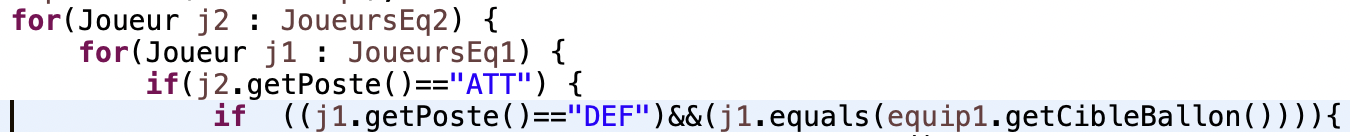
\includegraphics[width=15cm]{images/code_marquage.png}
\label{fig:marquage}
\end{figure}
       
\paragraph{}
    Avec le code \ref{fig:marquage}, les attaquants effectueront les déplacements vers les défenseurs uniquement en cas de possession de la balle d'un défenseur.

\paragraph{}
    Ensuite, lors d'un changement de possession de la balle, soit lors d'une interception par exemple, l'équipe dépossédée du ballon va se repositionner en bloc, via l'appel d'une méthode permettant le replacement d'un joueur dans sa zone tactique, déterminée par la composition choisie au préalable. En parallèle de ça, le bloc redescendra sur le terrain, afin de se repositionner de façon défensive. Et vice versa, l'équipe qui récupère le ballon elle, va monter sur le terrain afin de se mettre en position offensive, en bloc haut.
\paragraph{D2placement Gardien}
       En ce qui concerne les déplacements des gardiens, ils sont les mêmes pour les deux gardiens. Lorsque le ballon arrive a une certaine distance des buts, le gardien se positionnera dans l'axe du ballon afin d'être suffisamment bien placé lors d'un tir.

\begin{figure}[h]
\centering
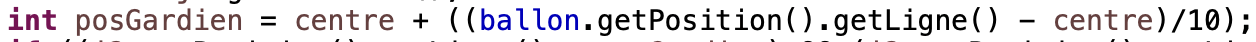
\includegraphics[width=15cm]{images/code_posgardien.png}
\label{fig:posGardien}
\end{figure}

\paragraph{}
   De plus, lorsque le ballon est situé dans une zone de 20 cases devant les buts, le gardien s'alignera avec la balle, en essayant de se mettre sur la même case que cette dernière afin de maximiser ses chances de l'arrêter.
\begin{figure}[h]
\centering
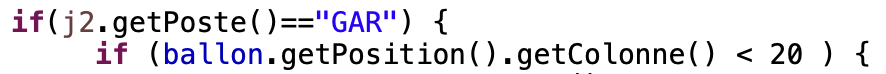
\includegraphics[width=10cm]{images/code_gardien.png}
\label{fig:gardien}
\end{figure}

\paragraph{Cas Particulier}
    Il existe un cas particulier lors de l'apparition de certaines actions spéciales. Le  cas du replacement du joueur qui réalise un corner ou une sortie de but.

\paragraph{}
    En effet, lorsqu'un joueur réalise ce genre d'action, il n'est plus positionné dans sa zone tactique, zone dans laquelle il réalise des déplacement. De ce fait, lors de l'arrivée de tel cas dans Manager, on récupère le joueur dans une variable centreur puis on l'oblige a se déplacer jusqu'à sa zone tactique ce qui empêche le joueur de rester bloque à l'endroit de son action jusqu'au prochain changement de possession.
    
\subsection{Solution IHM Graphique}

\paragraph{}
    On regroupera ici les solutions implémentées intéressante pour l'interface graphique du logiciel, selon les conceptions énoncés dans la section \ref{sec:conceptGraph}.

\paragraph{Choix Joueurs}
    Une des solutions intéressantes de notre IHM Graphique me semble être notre façon de gérer la sélection des Joueurs.

\paragraph{}
    La solution que l'on a implémenter diffère de notre conception, en effet, la sélection ne se fait plus dans la même fenêtre mais dans une fenêtre pour chaque poste. Et pour accéder aux différents postes, cela va se faire en fonction du constructeur choisi en fonction du nombre d'ArrayList donne en paramètre qui représentent les postes où les joueurs ont déjà étés sélectionnés.
    
\paragraph{}
    Ensuite, une fois le poste à remplir déterminer, pour que la sélection des joueurs soit visuel, il y a l'apparition des joueurs générer dans un JPanel à gauche sous forme de JLabel puis avec un MouseListener qui agit sur les JLabel, on les transfert sur le JPanel des Joueurs sélectionner à droite tout en vérifiant que l'on ne dépasse pas le nombre de joueur donner par le composition de l'équipe définit précédemment par l'utilisateur.

\paragraph{Statistique}
    Un autre élément important de notre IHM Graphique est la gestion et générations des statistiques. Pour décrire cela, on va d'abord détailler la récolte des informations puis la génération et l'affichage des graphiques.
    
\paragraph{}
    Pour la récolte des données, on récupère deux données. D'abord, lors de la création du terrain et l'affichage du match, on visite tous les joueurs des deux équipes pour calculer la moyenne de toutes les statistiques des joueurs puis dans ChartManager on génère un histogramme grâce à JFreeChart puis on le retourne dans un ChartPanel pour l'afficher sur l'écran. Ensuite, la seconde récolte de donnée se situe dans Manager pour récupérer toutes les occurrences des actions réalisé pendant le match. Ces informations seront exploitées lors de l'écran final de notre jeu comme un comparatif des actions réalise par les deux équipes.
    